\SourceLeaf{300}
auch in seiner Géométrie, Note X, wo er auch unrichtig \textsc{Lexell} citirt, und \textsc{Grunert} in der Fortsetzung von \textsc{Klügels} Wörterbuch, Artikel Trigonometrie (gleichfalls unrichtige Citation \textsc{Lexells}. Sie scheinen aus \textsc{Legendre} abgeschrieben zu haben).

\textsc{Clausen} hat mich gebeten, Ihnen seine Auflösung vorzulegen. Es folgt daraus, dass die Mittelpunkte der beiden andern Seiten des Dreiecks (die Basis ist die dritte) auf grössten Kreisen liegen, und die einfache Construction um den Pol des Ortkreises zu finden:

\begin{quote}
Man halbire die beiden andern Seiten und lasse aus den Halbirungspunkten Bögen von $90^0$ sich schneiden. Ihr Durchschnittspunkt ist der gesuchte Pol des kleinen Kreises, in dem die Spitzen der Dreiecke liegen.
\end{quote}

Ist diess durch geometrische Betrachtungen schon gefunden? \mbox{.\,.\,.\,.\,.\,.\,.\,.}\}

\medskip

\Needspace{6\baselineskip}
\begin{center}
\textsc{Gauss} an \textsc{Schumacher}. Göttingen, 6. Januar 1842.
\end{center}

\mbox{.\,.\,.\,.\,.\,.\,.} Bei der ganzen Sache war mir nur das merkwürdig gewesen, dass die analytische Angriffsarbeit diessmal so sehr viel weitschweifiger wird als der synthetische Beweis des Satzes, wenn man ihn schon hat. Ich selbst hatte mir das Resultat so enunciirt: man verbinde die Mitten der zwei Seiten des vorgegebenen Dreiecks (indem man die gegebene Basis die dritte Seite nennt) durch einen grössten Kreis; der damit durch die Spitze des Dreiecks parallel gezogene kleine Kreis ist der gesuchte geometrische Ort. Dass damit der Aufgabe genügt wird, ist in der That unmittelbar zu übersehen.

\Needspace{20\baselineskip}
\begin{center}\resizebox{7.3cm}{!}{%
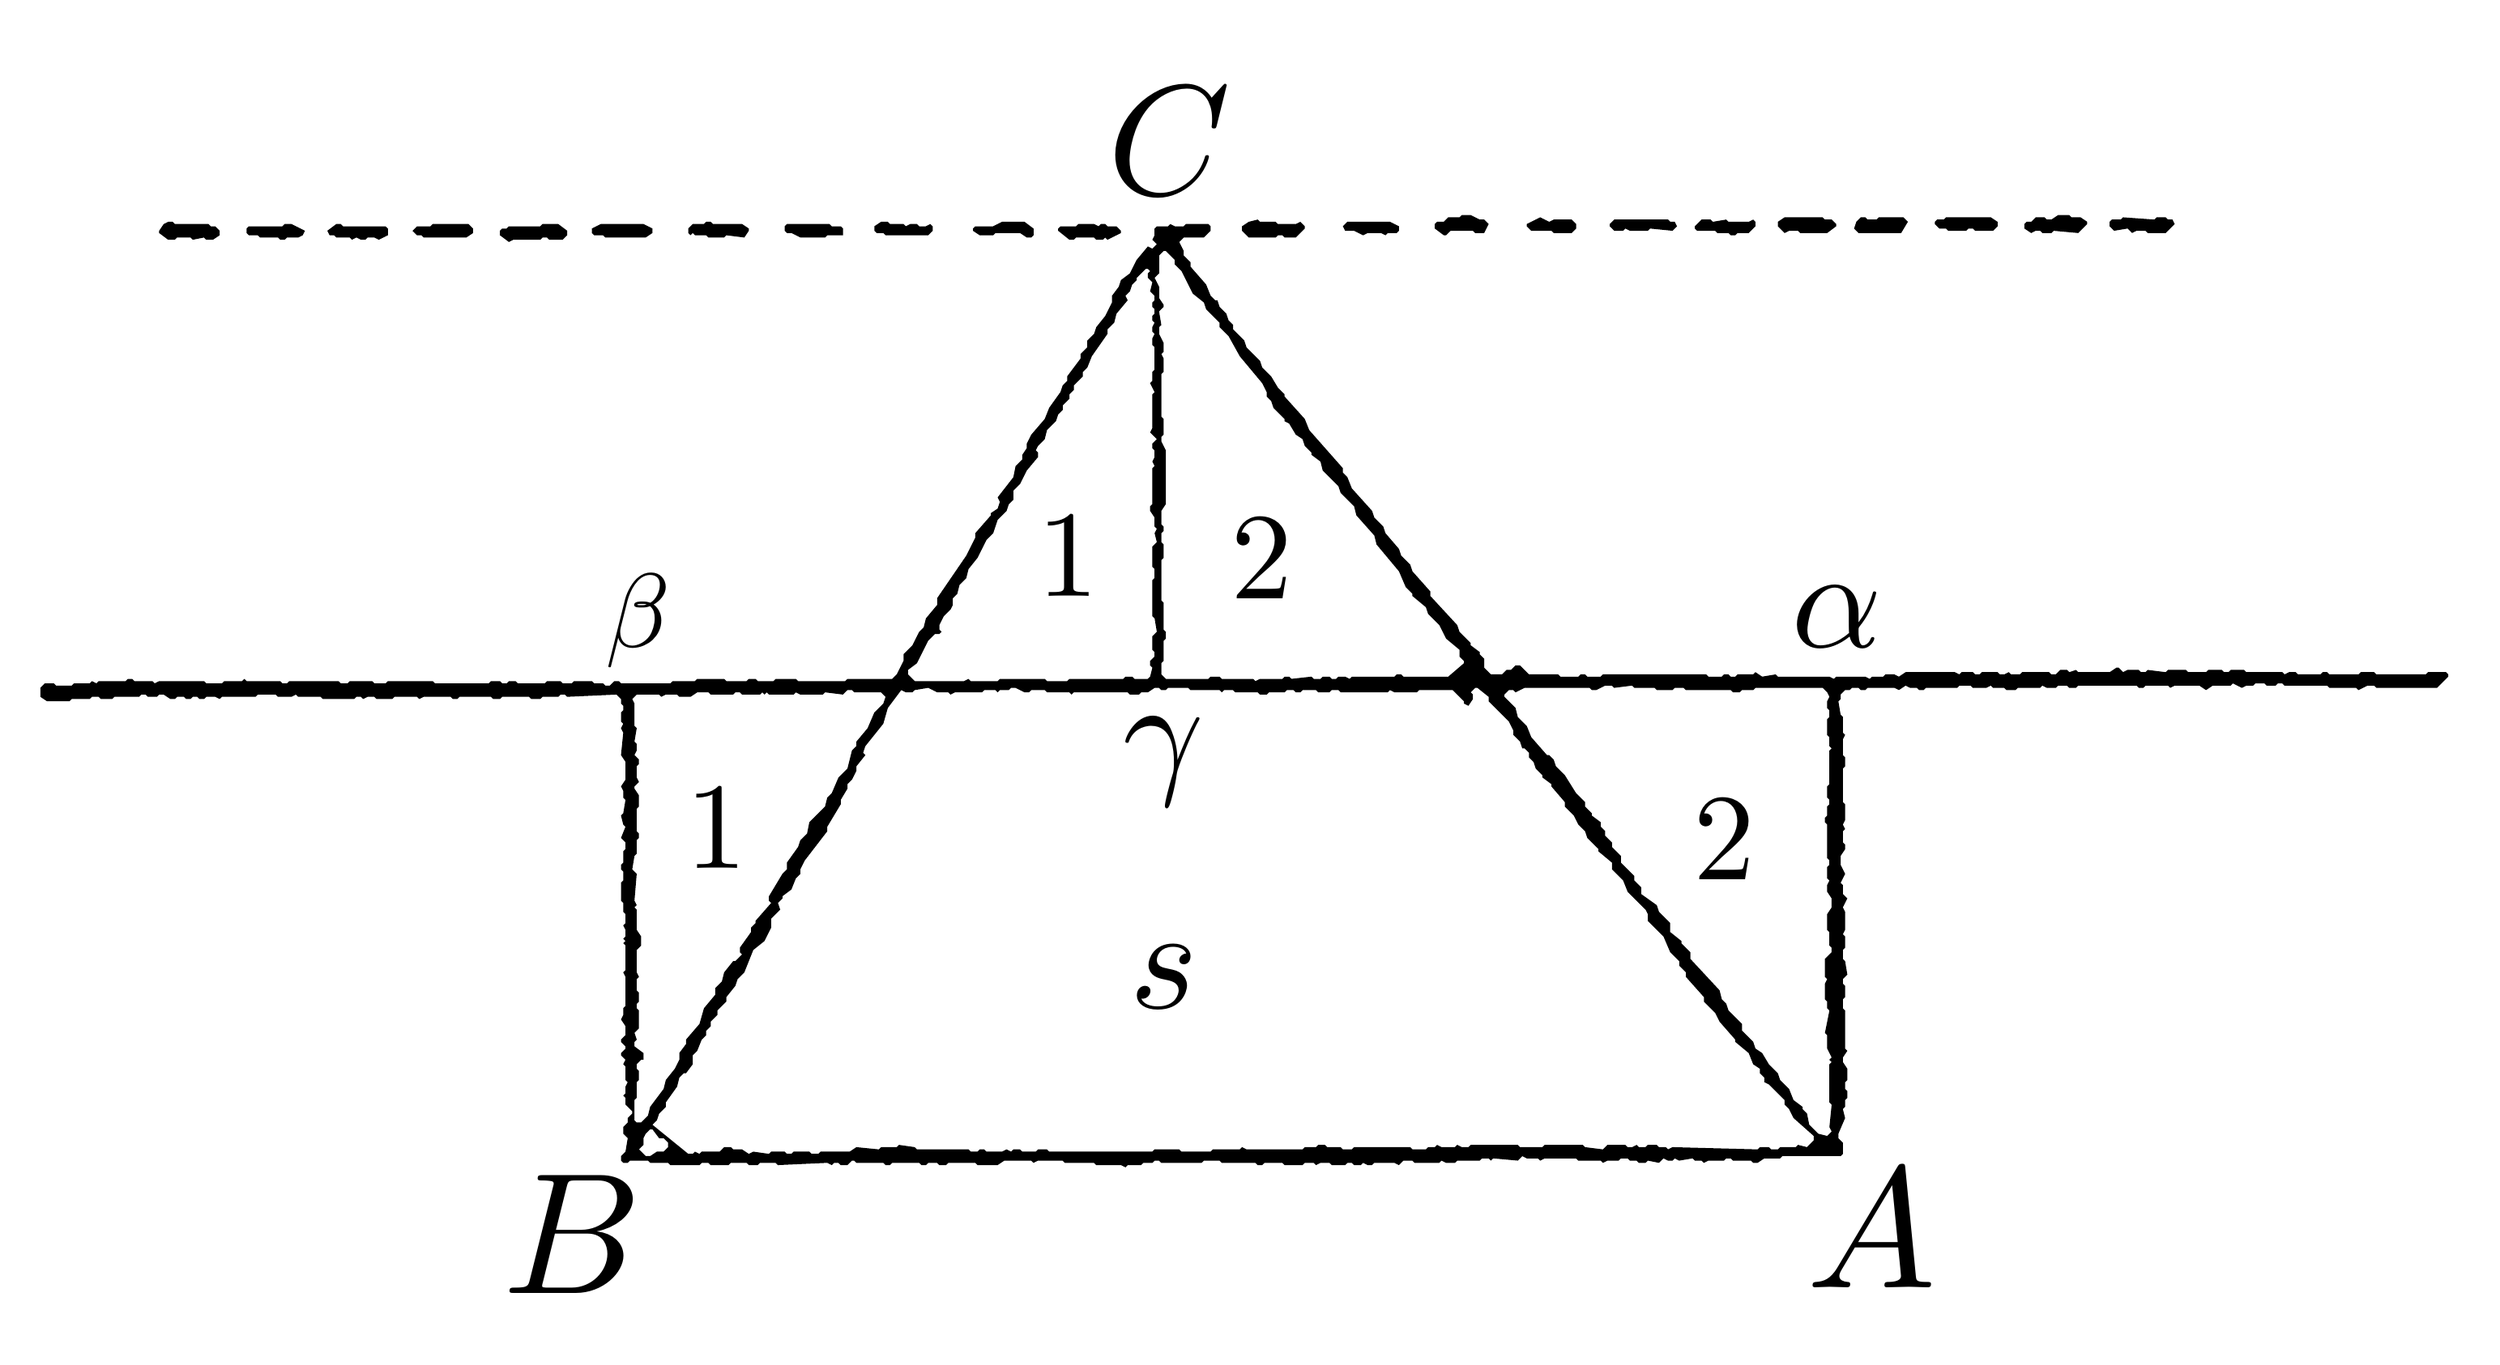
\begin{tikzpicture}[x=1pt,y=-1pt]
\path[use as bounding box] (0,0) rectangle (1095,589);
\path[fill=black,draw=none,even odd rule]
(8,301) -- (11,303) -- (21,303) -- (22,302) -- (30,302) -- (31,301) -- (34,301) -- (35,302) -- (40,302) -- (41,301) -- (52,301) -- (53,300) -- (55,300) -- (56,301) -- (60,301) -- (61,300) -- (63,300) -- (66,302) -- (68,302) -- (69,301) -- (72,301) -- (73,302) -- (75,302) -- (76,301) -- (78,301) -- (79,302) -- (81,302) -- (82,301) -- (86,301) -- (88,302) -- (89,301) -- (104,301) -- (105,300) -- (113,300) -- (114,301) -- (120,301) -- (122,300) -- (123,301) -- (133,301) -- (134,302) -- (148,302) -- (149,301) -- (151,301) -- (152,302) -- (154,301) -- (157,301) -- (158,302) -- (165,302) -- (166,301) -- (176,301) -- (177,302) -- (179,301) -- (191,301) -- (192,302) -- (194,302) -- (195,301) -- (209,301) -- (210,302) -- (213,302) -- (214,301) -- (226,301) -- (227,302) -- (231,302) -- (232,301) -- (239,301) -- (240,300) -- (242,300) -- (243,301) -- (265,300) -- (267,302) -- (267,304) -- (268,305) -- (268,307) -- (267,308) -- (267,312) -- (268,313) -- (267,315) -- (268,317) -- (267,327) -- (269,330) -- (269,338) -- (267,341) -- (268,343) -- (268,346) -- (269,347) -- (268,353) -- (267,354) -- (268,358) -- (269,359) -- (267,364) -- (269,366) -- (269,369) -- (268,370) -- (268,375) -- (267,376) -- (267,378) -- (268,379) -- (268,383) -- (267,384) -- (267,392) -- (268,393) -- (268,397) -- (269,398) -- (269,402) -- (268,403) -- (269,405) -- (269,408) -- (268,409) -- (269,410) -- (268,411) -- (269,412) -- (269,423) -- (268,424) -- (269,426) -- (269,439) -- (268,440) -- (268,443) -- (267,445) -- (269,448) -- (269,452) -- (267,454) -- (267,455) -- (269,457) -- (269,458) -- (267,460) -- (267,461) -- (269,463) -- (268,465) -- (269,466) -- (269,472) -- (270,473) -- (269,475) -- (269,478) -- (268,479) -- (269,480) -- (269,483) -- (272,486) -- (272,487) -- (270,489) -- (270,491) -- (268,493) -- (268,496) -- (270,498) -- (269,504) -- (267,506) -- (267,508) -- (268,509) -- (270,509) -- (271,508) -- (279,508) -- (280,509) -- (288,509) -- (289,510) -- (302,510) -- (303,509) -- (306,509) -- (307,510) -- (315,510) -- (316,509) -- (323,509) -- (324,510) -- (328,510) -- (329,509) -- (336,509) -- (337,510) -- (359,509) -- (361,510) -- (362,509) -- (364,509) -- (365,510) -- (368,510) -- (370,508) -- (371,508) -- (372,509) -- (384,509) -- (385,510) -- (387,510) -- (388,509) -- (400,509) -- (401,510) -- (403,510) -- (404,509) -- (408,509) -- (409,510) -- (412,510) -- (413,509) -- (425,509) -- (426,510) -- (435,510) -- (438,508) -- (450,508) -- (451,509) -- (453,508) -- (464,508) -- (465,509) -- (478,509) -- (479,510) -- (490,510) -- (492,511) -- (493,510) -- (499,510) -- (500,509) -- (504,509) -- (505,508) -- (507,508) -- (508,509) -- (526,509) -- (527,508) -- (534,508) -- (535,509) -- (550,509) -- (551,510) -- (553,510) -- (554,509) -- (562,509) -- (563,510) -- (571,510) -- (572,509) -- (576,509) -- (577,510) -- (579,509) -- (583,509) -- (584,510) -- (590,510) -- (591,509) -- (593,509) -- (594,510) -- (597,510) -- (598,509) -- (600,510) -- (602,510) -- (603,509) -- (612,509) -- (614,510) -- (616,508) -- (620,508) -- (621,509) -- (632,509) -- (633,508) -- (635,509) -- (639,509) -- (640,508) -- (650,508) -- (651,507) -- (654,507) -- (655,508) -- (656,507) -- (667,508) -- (669,506) -- (671,507) -- (676,507) -- (677,508) -- (679,507) -- (693,507) -- (694,508) -- (704,508) -- (705,509) -- (707,508) -- (712,508) -- (713,507) -- (716,507) -- (717,508) -- (720,508) -- (721,509) -- (724,509) -- (725,508) -- (730,509) -- (732,507) -- (734,508) -- (736,508) -- (737,507) -- (739,508) -- (745,507) -- (746,508) -- (749,508) -- (750,509) -- (752,508) -- (759,508) -- (760,507) -- (762,507) -- (763,508) -- (771,508) -- (772,509) -- (774,509) -- (777,507) -- (784,507) -- (785,506) -- (811,506) -- (812,505) -- (812,500) -- (810,498) -- (810,496) -- (813,489) -- (812,485) -- (813,484) -- (813,481) -- (814,480) -- (814,477) -- (813,476) -- (813,473) -- (814,472) -- (814,467) -- (812,464) -- (812,462) -- (814,459) -- (813,458) -- (813,441) -- (812,440) -- (812,436) -- (813,435) -- (813,430) -- (812,429) -- (812,427) -- (814,425) -- (813,419) -- (812,418) -- (812,414) -- (813,413) -- (813,408) -- (812,407) -- (813,405) -- (813,397) -- (812,395) -- (814,391) -- (812,389) -- (812,385) -- (811,384) -- (813,380) -- (811,376) -- (811,372) -- (813,369) -- (813,367) -- (812,366) -- (812,361) -- (813,360) -- (812,358) -- (813,356) -- (813,349) -- (812,348) -- (812,333) -- (813,332) -- (813,328) -- (812,327) -- (812,320) -- (813,318) -- (812,317) -- (812,310) -- (811,309) -- (810,303) -- (811,302) -- (811,300) -- (813,298) -- (815,298) -- (816,297) -- (819,297) -- (820,298) -- (822,298) -- (823,297) -- (835,297) -- (837,298) -- (840,296) -- (842,297) -- (845,297) -- (846,298) -- (848,298) -- (849,297) -- (863,297) -- (864,296) -- (869,296) -- (870,297) -- (876,297) -- (878,296) -- (879,297) -- (884,297) -- (885,298) -- (889,298) -- (890,297) -- (900,297) -- (901,296) -- (903,297) -- (907,297) -- (908,296) -- (912,296) -- (913,297) -- (916,297) -- (917,296) -- (943,296) -- (944,297) -- (946,297) -- (947,296) -- (957,296) -- (958,297) -- (960,296) -- (971,296) -- (974,298) -- (977,296) -- (985,296) -- (986,295) -- (990,297) -- (992,296) -- (995,296) -- (996,295) -- (1000,295) -- (1001,296) -- (1005,296) -- (1006,295) -- (1008,295) -- (1009,296) -- (1028,296) -- (1029,297) -- (1041,297) -- (1042,298) -- (1046,296) -- (1049,296) -- (1050,297) -- (1077,297) -- (1082,292) -- (1082,291) -- (1081,290) -- (1073,290) -- (1072,291) -- (1050,291) -- (1049,290) -- (1043,290) -- (1042,291) -- (1029,291) -- (1028,290) -- (1026,290) -- (1025,291) -- (1015,291) -- (1014,290) -- (1011,290) -- (1009,291) -- (1008,290) -- (992,290) -- (991,289) -- (985,289) -- (984,290) -- (982,290) -- (981,289) -- (975,289) -- (974,290) -- (966,290) -- (965,289) -- (957,289) -- (956,290) -- (948,289) -- (947,290) -- (945,290) -- (944,289) -- (939,289) -- (937,290) -- (935,288) -- (934,288) -- (931,290) -- (917,290) -- (916,289) -- (913,290) -- (912,289) -- (909,289) -- (907,291) -- (905,291) -- (904,290) -- (892,290) -- (891,291) -- (887,291) -- (886,290) -- (884,291) -- (882,291) -- (881,290) -- (874,290) -- (873,291) -- (871,291) -- (870,290) -- (865,290) -- (864,291) -- (862,290) -- (840,290) -- (837,292) -- (835,291) -- (831,291) -- (830,292) -- (825,292) -- (824,293) -- (822,292) -- (809,292) -- (808,293) -- (806,292) -- (783,292) -- (782,291) -- (776,292) -- (773,290) -- (772,291) -- (765,291) -- (764,292) -- (762,292) -- (761,291) -- (759,291) -- (758,292) -- (752,292) -- (751,291) -- (705,291) -- (704,292) -- (698,292) -- (697,291) -- (695,291) -- (694,292) -- (686,292) -- (685,291) -- (672,291) -- (668,287) -- (666,287) -- (664,289) -- (662,289) -- (660,291) -- (655,291) -- (652,288) -- (652,284) -- (650,282) -- (650,281) -- (646,278) -- (646,277) -- (641,272) -- (640,269) -- (628,256) -- (628,254) -- (620,245) -- (619,242) -- (615,238) -- (614,235) -- (608,228) -- (607,225) -- (603,221) -- (602,218) -- (593,208) -- (591,203) -- (589,201) -- (589,199) -- (574,182) -- (572,177) -- (563,167) -- (563,166) -- (560,163) -- (557,158) -- (553,154) -- (552,151) -- (546,145) -- (545,142) -- (540,137) -- (540,135) -- (538,133) -- (537,130) -- (534,127) -- (533,124) -- (532,124) -- (530,122) -- (528,117) -- (521,109) -- (521,107) -- (518,104) -- (518,102) -- (516,98) -- (518,96) -- (527,96) -- (530,93) -- (530,91) -- (529,90) -- (519,90) -- (518,91) -- (514,91) -- (512,90) -- (511,91) -- (506,91) -- (505,92) -- (505,95) -- (504,97) -- (506,99) -- (504,101) -- (502,100) -- (497,106) -- (494,112) -- (490,115) -- (489,118) -- (486,122) -- (486,125) -- (483,131) -- (479,136) -- (478,139) -- (475,142) -- (475,145) -- (472,148) -- (472,150) -- (466,158) -- (466,160) -- (464,162) -- (463,165) -- (458,172) -- (456,177) -- (450,184) -- (448,188) -- (448,190) -- (446,193) -- (446,195) -- (443,198) -- (442,203) -- (435,212) -- (436,214) -- (435,217) -- (432,219) -- (432,220) -- (425,228) -- (425,230) -- (421,238) -- (408,257) -- (408,260) -- (403,266) -- (402,270) -- (400,272) -- (397,278) -- (393,282) -- (393,285) -- (390,291) -- (388,293) -- (368,293) -- (367,294) -- (346,294) -- (345,293) -- (336,293) -- (335,294) -- (328,294) -- (327,293) -- (324,293) -- (323,294) -- (314,294) -- (313,293) -- (301,293) -- (300,294) -- (290,294) -- (289,295) -- (267,295) -- (266,294) -- (264,294) -- (262,296) -- (260,296) -- (259,295) -- (255,295) -- (254,294) -- (246,294) -- (245,295) -- (241,295) -- (240,294) -- (234,294) -- (233,295) -- (221,295) -- (220,294) -- (217,294) -- (216,295) -- (214,295) -- (213,294) -- (209,294) -- (208,295) -- (184,295) -- (183,294) -- (163,294) -- (162,295) -- (157,295) -- (156,294) -- (146,294) -- (145,295) -- (142,295) -- (141,294) -- (119,294) -- (118,295) -- (116,295) -- (115,294) -- (100,294) -- (99,293) -- (98,294) -- (90,294) -- (89,295) -- (82,295) -- (81,294) -- (61,294) -- (59,295) -- (58,294) -- (50,294) -- (49,293) -- (47,293) -- (46,294) -- (34,294) -- (33,295) -- (31,294) -- (30,295) -- (23,295) -- (22,296) -- (15,296) -- (14,295) -- (10,295) -- (8,297) -- cycle
(281,494) -- (284,498) -- (286,498) -- (288,500) -- (288,502) -- (286,504) -- (283,504) -- (280,506) -- (278,506) -- (275,503) -- (277,501) -- (277,498) -- (278,496) -- (280,494) -- cycle
(383,299) -- (385,301) -- (384,304) -- (380,308) -- (377,315) -- (372,321) -- (372,323) -- (370,325) -- (368,333) -- (364,337) -- (361,344) -- (359,346) -- (358,350) -- (351,357) -- (350,362) -- (347,365) -- (346,368) -- (341,375) -- (341,378) -- (339,380) -- (333,390) -- (333,392) -- (334,393) -- (327,401) -- (327,402) -- (325,404) -- (325,406) -- (320,413) -- (320,415) -- (321,416) -- (318,419) -- (317,419) -- (313,424) -- (312,428) -- (309,431) -- (309,434) -- (304,440) -- (302,447) -- (296,454) -- (296,456) -- (293,460) -- (293,463) -- (291,467) -- (287,472) -- (286,476) -- (280,484) -- (279,488) -- (276,491) -- (274,491) -- (273,490) -- (273,481) -- (274,480) -- (274,473) -- (275,472) -- (275,468) -- (274,467) -- (274,465) -- (276,463) -- (277,463) -- (277,460) -- (273,457) -- (273,455) -- (274,454) -- (273,451) -- (275,449) -- (275,441) -- (274,440) -- (274,438) -- (275,437) -- (275,433) -- (274,432) -- (274,427) -- (275,426) -- (274,424) -- (274,414) -- (276,412) -- (276,408) -- (274,405) -- (274,396) -- (273,395) -- (274,394) -- (273,392) -- (274,380) -- (272,378) -- (273,372) -- (274,371) -- (274,365) -- (275,364) -- (275,362) -- (274,361) -- (274,351) -- (275,350) -- (275,345) -- (273,342) -- (273,341) -- (275,339) -- (274,337) -- (274,332) -- (275,331) -- (275,329) -- (273,327) -- (274,325) -- (274,322) -- (273,321) -- (274,315) -- (273,314) -- (273,304) -- (272,302) -- (274,300) -- (284,300) -- (285,301) -- (287,300) -- (292,300) -- (293,301) -- (298,301) -- (301,299) -- (306,299) -- (307,300) -- (317,300) -- (318,299) -- (320,299) -- (321,300) -- (329,300) -- (330,299) -- (331,300) -- (332,299) -- (333,300) -- (344,300) -- (345,299) -- (347,300) -- (357,300) -- (358,299) -- (366,300) -- (368,298) -- (370,298) -- (371,299) -- cycle
(281,492) -- (283,490) -- (284,487) -- (287,484) -- (287,482) -- (292,475) -- (293,471) -- (295,469) -- (296,469) -- (299,465) -- (299,461) -- (301,459) -- (303,454) -- (305,452) -- (305,450) -- (307,448) -- (307,446) -- (310,443) -- (310,441) -- (314,437) -- (314,435) -- (318,430) -- (319,427) -- (322,424) -- (326,414) -- (331,410) -- (334,404) -- (334,400) -- (338,396) -- (337,393) -- (339,391) -- (339,390) -- (343,387) -- (345,382) -- (347,380) -- (347,378) -- (349,374) -- (359,361) -- (359,359) -- (365,349) -- (365,347) -- (368,342) -- (368,340) -- (370,338) -- (372,334) -- (372,332) -- (376,327) -- (375,326) -- (376,323) -- (384,313) -- (386,306) -- (392,298) -- (394,299) -- (397,299) -- (398,298) -- (404,297) -- (408,299) -- (413,299) -- (414,300) -- (416,299) -- (428,299) -- (429,298) -- (434,298) -- (435,299) -- (436,298) -- (440,298) -- (441,297) -- (443,297) -- (447,299) -- (449,299) -- (450,298) -- (456,298) -- (457,299) -- (467,299) -- (468,300) -- (469,299) -- (493,299) -- (494,300) -- (498,300) -- (499,299) -- (502,299) -- (505,297) -- (507,297) -- (508,298) -- (510,298) -- (511,297) -- (520,297) -- (521,298) -- (534,298) -- (535,299) -- (536,298) -- (540,298) -- (541,299) -- (551,299) -- (552,300) -- (555,300) -- (556,299) -- (563,299) -- (564,298) -- (567,298) -- (568,299) -- (570,299) -- (571,298) -- (577,298) -- (578,299) -- (583,299) -- (584,298) -- (587,298) -- (588,299) -- (609,299) -- (610,298) -- (612,299) -- (622,299) -- (623,298) -- (638,298) -- (643,303) -- (643,304) -- (645,305) -- (647,302) -- (647,300) -- (646,299) -- (648,297) -- (649,297) -- (654,301) -- (654,303) -- (663,312) -- (665,316) -- (665,318) -- (668,321) -- (669,324) -- (670,324) -- (672,326) -- (672,328) -- (674,330) -- (675,333) -- (678,336) -- (678,337) -- (682,340) -- (682,341) -- (688,348) -- (688,350) -- (692,354) -- (694,358) -- (697,361) -- (698,364) -- (703,369) -- (703,370) -- (709,375) -- (709,378) -- (714,383) -- (716,388) -- (724,396) -- (725,398) -- (725,401) -- (732,408) -- (735,415) -- (739,419) -- (739,421) -- (742,424) -- (742,426) -- (750,435) -- (750,437) -- (755,442) -- (757,446) -- (764,454) -- (764,455) -- (770,460) -- (772,465) -- (775,467) -- (775,469) -- (777,471) -- (777,473) -- (779,474) -- (786,481) -- (786,483) -- (788,485) -- (790,489) -- (799,497) -- (799,499) -- (796,502) -- (792,501) -- (791,502) -- (784,502) -- (783,503) -- (780,503) -- (779,502) -- (775,502) -- (774,503) -- (736,502) -- (734,503) -- (733,502) -- (730,502) -- (729,501) -- (725,501) -- (724,502) -- (721,502) -- (720,501) -- (718,502) -- (716,502) -- (715,501) -- (707,501) -- (705,503) -- (697,502) -- (696,501) -- (679,501) -- (678,502) -- (668,502) -- (667,501) -- (646,501) -- (645,502) -- (642,502) -- (640,501) -- (639,502) -- (633,502) -- (631,501) -- (630,502) -- (627,502) -- (626,503) -- (620,503) -- (619,502) -- (594,502) -- (593,503) -- (589,503) -- (588,502) -- (582,502) -- (581,501) -- (578,501) -- (577,502) -- (572,502) -- (571,503) -- (546,503) -- (544,502) -- (543,503) -- (531,503) -- (530,504) -- (517,504) -- (516,503) -- (505,503) -- (504,504) -- (458,504) -- (457,503) -- (453,503) -- (452,504) -- (446,504) -- (445,503) -- (442,503) -- (441,504) -- (439,503) -- (437,504) -- (430,504) -- (429,503) -- (427,503) -- (426,504) -- (423,504) -- (422,503) -- (399,503) -- (398,502) -- (391,501) -- (390,502) -- (383,502) -- (382,503) -- (372,502) -- (369,504) -- (356,504) -- (355,505) -- (352,505) -- (351,504) -- (344,504) -- (343,505) -- (341,505) -- (340,504) -- (334,504) -- (333,505) -- (326,504) -- (324,505) -- (321,503) -- (317,503) -- (316,502) -- (313,502) -- (311,504) -- (303,504) -- (302,505) -- (300,504) -- (299,505) -- (297,505) -- cycle
(663,298) -- (665,298) -- (666,299) -- (670,297) -- (699,297) -- (700,298) -- (702,298) -- (706,296) -- (709,296) -- (710,297) -- (718,296) -- (719,297) -- (728,297) -- (729,298) -- (736,298) -- (737,297) -- (741,297) -- (742,298) -- (762,298) -- (763,299) -- (766,299) -- (767,298) -- (772,298) -- (773,297) -- (803,297) -- (805,299) -- (806,301) -- (805,303) -- (805,306) -- (806,307) -- (806,310) -- (805,311) -- (805,318) -- (806,319) -- (806,323) -- (807,324) -- (806,325) -- (806,340) -- (805,341) -- (805,346) -- (806,347) -- (806,349) -- (805,350) -- (805,354) -- (804,355) -- (804,357) -- (805,358) -- (805,373) -- (806,374) -- (806,376) -- (805,377) -- (805,382) -- (806,383) -- (805,385) -- (805,388) -- (807,391) -- (807,395) -- (805,398) -- (805,405) -- (806,406) -- (806,412) -- (807,413) -- (807,415) -- (804,418) -- (804,426) -- (805,427) -- (804,429) -- (804,436) -- (805,437) -- (805,440) -- (806,441) -- (804,451) -- (805,452) -- (805,458) -- (807,462) -- (806,463) -- (807,464) -- (806,465) -- (806,482) -- (807,483) -- (806,493) -- (807,495) -- (805,497) -- (801,496) -- (797,492) -- (796,487) -- (794,485) -- (794,484) -- (790,481) -- (788,476) -- (784,472) -- (783,469) -- (779,465) -- (776,460) -- (773,458) -- (772,455) -- (767,450) -- (767,447) -- (761,441) -- (760,438) -- (758,436) -- (757,432) -- (744,418) -- (744,415) -- (740,411) -- (740,410) -- (735,406) -- (735,402) -- (730,397) -- (729,394) -- (722,389) -- (722,386) -- (719,383) -- (719,381) -- (713,375) -- (713,372) -- (709,368) -- (709,366) -- (706,363) -- (706,361) -- (704,359) -- (704,357) -- (700,354) -- (700,353) -- (697,350) -- (697,348) -- (693,344) -- (688,336) -- (684,332) -- (683,329) -- (681,327) -- (680,327) -- (673,319) -- (671,314) -- (667,310) -- (666,306) -- (661,301) -- (661,300) -- cycle
(502,110) -- (503,111) -- (502,112) -- (502,114) -- (504,116) -- (503,120) -- (505,122) -- (505,124) -- (504,125) -- (504,127) -- (505,128) -- (505,130) -- (504,131) -- (504,133) -- (505,134) -- (504,136) -- (504,138) -- (505,139) -- (504,141) -- (504,144) -- (505,145) -- (505,155) -- (504,156) -- (504,160) -- (503,161) -- (505,165) -- (504,166) -- (504,181) -- (503,183) -- (506,186) -- (504,188) -- (504,190) -- (505,191) -- (505,194) -- (504,196) -- (505,198) -- (504,199) -- (504,215) -- (503,216) -- (503,218) -- (505,221) -- (505,225) -- (506,226) -- (505,228) -- (506,232) -- (504,234) -- (504,243) -- (505,244) -- (505,248) -- (504,249) -- (504,265) -- (505,266) -- (506,272) -- (504,274) -- (504,280) -- (505,281) -- (505,283) -- (503,285) -- (503,287) -- (504,288) -- (503,292) -- (502,293) -- (496,293) -- (495,292) -- (492,292) -- (491,293) -- (467,293) -- (466,294) -- (457,294) -- (456,293) -- (436,293) -- (435,294) -- (423,294) -- (422,293) -- (420,294) -- (398,294) -- (395,291) -- (395,289) -- (399,286) -- (404,276) -- (407,273) -- (409,273) -- (410,272) -- (409,271) -- (409,269) -- (411,265) -- (414,262) -- (415,260) -- (415,257) -- (417,255) -- (418,251) -- (421,248) -- (422,244) -- (426,239) -- (430,231) -- (433,228) -- (435,222) -- (439,218) -- (440,215) -- (442,213) -- (442,209) -- (445,206) -- (448,200) -- (453,194) -- (453,192) -- (452,191) -- (453,189) -- (456,186) -- (457,182) -- (461,178) -- (462,175) -- (464,173) -- (464,171) -- (467,168) -- (467,166) -- (469,164) -- (469,162) -- (473,158) -- (473,156) -- (475,154) -- (477,149) -- (484,139) -- (484,137) -- (487,134) -- (488,130) -- (493,124) -- (492,122) -- (494,120) -- (495,117) -- (497,115) -- (497,114) -- (501,110) -- cycle
(509,102) -- (510,102) -- (514,106) -- (514,108) -- (517,111) -- (522,121) -- (527,125) -- (528,128) -- (534,134) -- (534,136) -- (538,140) -- (543,149) -- (553,161) -- (555,165) -- (555,167) -- (557,169) -- (558,172) -- (563,177) -- (563,178) -- (565,179) -- (568,184) -- (571,186) -- (572,189) -- (575,192) -- (575,193) -- (579,196) -- (580,200) -- (587,207) -- (588,210) -- (594,216) -- (595,220) -- (603,229) -- (604,233) -- (614,245) -- (617,252) -- (620,255) -- (620,256) -- (626,261) -- (627,264) -- (632,269) -- (635,275) -- (641,280) -- (641,283) -- (643,285) -- (643,286) -- (636,292) -- (616,292) -- (615,291) -- (613,291) -- (612,292) -- (593,292) -- (592,293) -- (590,292) -- (587,292) -- (586,293) -- (584,293) -- (583,292) -- (580,292) -- (579,293) -- (576,293) -- (575,292) -- (566,293) -- (565,292) -- (563,292) -- (562,293) -- (552,293) -- (550,294) -- (549,293) -- (535,293) -- (534,292) -- (530,292) -- (529,293) -- (510,293) -- (508,291) -- (508,286) -- (509,285) -- (509,276) -- (510,275) -- (510,272) -- (509,271) -- (509,259) -- (508,258) -- (508,240) -- (509,239) -- (509,233) -- (508,232) -- (508,228) -- (509,227) -- (509,225) -- (508,224) -- (508,218) -- (510,215) -- (510,191) -- (508,187) -- (508,185) -- (509,184) -- (509,177) -- (508,176) -- (508,157) -- (509,156) -- (509,150) -- (508,148) -- (509,147) -- (509,143) -- (507,139) -- (507,136) -- (508,135) -- (507,129) -- (509,127) -- (509,126) -- (507,123) -- (507,118) -- (505,114) -- (507,112) -- (507,104) -- cycle
(462,92) -- (462,93) -- (467,97) -- (469,97) -- (470,96) -- (478,96) -- (479,97) -- (482,97) -- (483,96) -- (484,97) -- (490,94) -- (490,93) -- (488,91) -- (484,91) -- (483,90) -- (481,90) -- (480,91) -- (478,90) -- (471,90) -- (470,91) -- (463,91) -- cycle
(340,91) -- (340,93) -- (341,94) -- (343,94) -- (347,96) -- (358,96) -- (359,95) -- (366,95) -- (366,92) -- (365,91) -- (361,91) -- (360,90) -- (341,90) -- cycle
(254,92) -- (254,94) -- (255,95) -- (259,95) -- (260,96) -- (278,96) -- (281,94) -- (281,92) -- (277,90) -- (258,90) -- cycle
(243,93) -- (239,90) -- (232,90) -- (231,91) -- (217,91) -- (216,92) -- (214,92) -- (213,93) -- (213,95) -- (217,98) -- (219,97) -- (231,97) -- (232,96) -- (234,96) -- (235,97) -- (241,97) -- (243,95) -- cycle
(174,93) -- (176,95) -- (178,95) -- (179,96) -- (198,96) -- (201,94) -- (201,92) -- (199,90) -- (183,90) -- (182,91) -- (176,91) -- cycle
(136,93) -- (137,95) -- (139,95) -- (140,96) -- (146,96) -- (147,97) -- (149,96) -- (151,97) -- (153,97) -- (154,96) -- (157,96) -- (159,97) -- (163,95) -- (163,92) -- (162,91) -- (143,91) -- (142,90) -- (140,90) -- cycle
(126,93) -- (120,90) -- (117,90) -- (116,91) -- (101,91) -- (100,92) -- (100,94) -- (101,95) -- (105,95) -- (106,96) -- (114,96) -- (115,97) -- (117,97) -- (118,96) -- (123,96) -- (125,95) -- cycle
(589,91) -- (590,93) -- (594,93) -- (598,95) -- (600,94) -- (606,94) -- (608,95) -- (609,94) -- (613,94) -- (614,93) -- (614,91) -- (610,89) -- (591,89) -- cycle
(424,92) -- (424,93) -- (427,95) -- (433,95) -- (434,94) -- (445,94) -- (448,96) -- (450,96) -- (451,95) -- (451,92) -- (447,89) -- (437,89) -- (433,91) -- (425,91) -- cycle
(380,91) -- (380,93) -- (381,94) -- (384,94) -- (385,95) -- (404,95) -- (406,93) -- (406,91) -- (405,90) -- (403,91) -- (400,91) -- (399,90) -- (396,90) -- (394,91) -- (393,90) -- (387,90) -- (386,89) -- (383,89) -- cycle
(297,92) -- (297,94) -- (298,95) -- (299,94) -- (300,95) -- (305,95) -- (306,96) -- (313,96) -- (314,95) -- (322,96) -- (324,93) -- (324,92) -- (321,90) -- (308,90) -- (307,89) -- (305,89) -- (304,90) -- (299,90) -- cycle
(61,93) -- (61,94) -- (65,97) -- (68,97) -- (69,96) -- (75,96) -- (76,97) -- (81,96) -- (82,97) -- (85,97) -- (88,95) -- (88,93) -- (86,91) -- (84,91) -- (83,90) -- (68,90) -- (67,89) -- (65,89) -- (63,90) -- cycle
(746,92) -- (747,93) -- (755,93) -- (756,94) -- (761,94) -- (762,95) -- (764,95) -- (765,94) -- (770,94) -- (773,91) -- (773,89) -- (772,88) -- (770,89) -- (761,89) -- (760,88) -- (754,89) -- (753,88) -- (749,88) -- (746,91) -- cycle
(708,90) -- (708,91) -- (710,93) -- (714,93) -- (715,92) -- (717,93) -- (725,93) -- (726,92) -- (736,93) -- (738,91) -- (737,89) -- (735,89) -- (734,88) -- (710,88) -- cycle
(544,91) -- (544,93) -- (547,96) -- (559,96) -- (560,95) -- (562,95) -- (563,96) -- (568,96) -- (572,92) -- (572,91) -- (570,89) -- (568,90) -- (560,90) -- (559,89) -- (552,89) -- (551,88) -- (547,89) -- cycle
(931,89) -- (931,91) -- (933,93) -- (939,92) -- (941,94) -- (943,93) -- (947,93) -- (948,94) -- (956,94) -- (960,90) -- (959,88) -- (957,88) -- (956,87) -- (952,87) -- (951,88) -- (937,87) -- (936,88) -- (932,88) -- cycle
(853,89) -- (853,90) -- (855,92) -- (858,92) -- (859,93) -- (867,93) -- (868,92) -- (870,92) -- (871,93) -- (879,93) -- (881,91) -- (881,89) -- (878,87) -- (858,87) -- (857,88) -- (854,88) -- cycle
(817,92) -- (819,94) -- (838,94) -- (841,89) -- (839,87) -- (828,87) -- (827,88) -- (823,88) -- (822,87) -- (820,87) -- (818,89) -- cycle
(783,89) -- (783,91) -- (786,94) -- (788,93) -- (792,93) -- (793,94) -- (805,94) -- (809,91) -- (809,90) -- (807,88) -- (804,88) -- (803,87) -- (786,87) -- cycle
(671,90) -- (671,91) -- (673,93) -- (682,93) -- (683,94) -- (691,94) -- (693,92) -- (693,90) -- (691,88) -- (683,88) -- (681,89) -- (677,87) -- cycle
(921,89) -- (918,87) -- (914,87) -- (913,86) -- (908,86) -- (905,88) -- (903,88) -- (902,87) -- (898,87) -- (896,89) -- (894,89) -- (893,90) -- (893,92) -- (896,94) -- (898,93) -- (900,93) -- (901,94) -- (905,94) -- (906,93) -- (917,94) -- (921,90) -- cycle
(654,90) -- (652,88) -- (650,88) -- (646,86) -- (642,86) -- (641,87) -- (636,87) -- (634,89) -- (631,89) -- (630,90) -- (630,92) -- (634,95) -- (635,95) -- (637,93) -- (647,93) -- (648,94) -- (652,94) -- cycle;
\node[inner sep=0pt,font=\fontsize{10}{10}\selectfont] at (511.5,53.0) {\scalebox{7.0}{$C$}};
\node[inner sep=0pt,font=\fontsize{10}{10}\selectfont] at (274.5,267.0) {\scalebox{4.7}{$\beta$}};
\node[inner sep=0pt,font=\fontsize{10}{10}\selectfont] at (809.5,265.5) {\scalebox{6.3}{$\alpha$}};
\node[inner sep=0pt,font=\fontsize{10}{10}\selectfont] at (509.0,330.0) {\scalebox{6.3}{$\gamma$}};
\node[inner sep=0pt,font=\fontsize{10}{10}\selectfont] at (466.5,238.5) {\scalebox{5.5}{$1$}};
\node[inner sep=0pt,font=\fontsize{10}{10}\selectfont] at (553.0,239.5) {\scalebox{5.5}{$2$}};
\node[inner sep=0pt,font=\fontsize{10}{10}\selectfont] at (309.5,360.0) {\scalebox{5.5}{$1$}};
\node[inner sep=0pt,font=\fontsize{10}{10}\selectfont] at (759.0,365.0) {\scalebox{5.5}{$2$}};
\node[inner sep=0pt,font=\fontsize{10}{10}\selectfont] at (509.0,426.0) {\scalebox{6.5}{$s$}};
\node[inner sep=0pt,font=\fontsize{10}{10}\selectfont] at (245.5,541.0) {\scalebox{7.7}{$B$}};
\node[inner sep=0pt,font=\fontsize{10}{10}\selectfont] at (825.0,538.5) {\scalebox{7.7}{$A$}};
\end{tikzpicture}%
}
\end{center}

Indem man nemlich auf den bemeldeten grössten Kreis die Perpendikel $A\alpha$, $B\beta$, $C\gamma$ fällt, bilden sich für nebenstehende Figur vier rechtwinklige Dreiecke $1,1,2,2$, wo die Gleichheit von $1=1$ und $2=2$ evident ist, also das Dreieck $ABC$ ist dem Viereck $A\alpha\beta B$ an Inhalt gleich; aber dieses Viereck ist von der Lage von $C$ in dem punktir%
